\documentclass{article}
\usepackage[margin=1in]{geometry}
\usepackage{amsmath,amsthm,amssymb}
\usepackage{bbm,enumerate,mathtools}
\usepackage{tikz,pgfplots}
\usepackage{chessboard}
\usepackage[hidelinks]{hyperref}
\usepackage{multicol} % Problem 35
\usepackage{xstring} % Difficulty command
\usetikzlibrary{shapes.geometric}

\newenvironment{question}{\begin{trivlist}\item[\textbf{Question.}]}{\end{trivlist}}
\newenvironment{note}{\begin{trivlist}\item[\textbf{Note.}]}{\end{trivlist}}
\newenvironment{references}{\begin{trivlist}\item[\textbf{References.}]}{\end{trivlist}}
\newenvironment{related}{\begin{trivlist}\item[\textbf{Related.}]\end{trivlist}\begin{enumerate}}{\end{enumerate}}

\newcommand\score[1]{
\pgfmathsetmacro\pgfxa{#1+1}
\tikzstyle{scorestars}=[
  star,
  star points=5,
  star point ratio=2.25,
  draw,
  inner sep=3pt,
  anchor=outer point 5
]
  \begin{tikzpicture}[baseline]
    \draw[opacity=0] (0,-0.5) rectangle (0,0.2); % Workaround for whitespace at the bottom.
    \foreach \i in {1,...,4} {
      \pgfmathparse{(\i<=#1?"yellow":"gray")}
      \edef\starcolor{\pgfmathresult}
      \draw (\i*4.5ex,0) node[name=star\i,scorestars,fill=\starcolor]  {};
    }
  \end{tikzpicture}
}

\newcommand{\difficulty}[1]{%
  \IfEqCase{#1}{%
      {1}{
        
\begin{tikzpicture}[scale=0.7, baseline=0.9mm]%
          \definecolor{slopegreen}{rgb}{0.0, 0.5, 0.0}%
          \fill[slopegreen] (0.5,0.5) circle (0.5);%
        \end{tikzpicture}%
      }%
      {2}{
        
\begin{tikzpicture}[scale=0.7, baseline=0.9mm]%
          \definecolor{slopeblue}{rgb}{0.0, 0.44, 1.00}
          \fill[slopeblue] (0,0) rectangle (1,1);%
        \end{tikzpicture}%
      }%
      {3}{
\begin{tikzpicture}[scale=0.7, baseline=0.9mm]\fill (0,0.5)--(0.5, 0)--(1,0.5)--(0.5,1)--cycle; \end{tikzpicture}}%
      {4}{
\begin{tikzpicture}[scale=0.7, baseline=0.9mm]\fill (0.25,0)--(0,0.5)--(0.25,1)--(0.5,0.5)--cycle; \fill (0.75,0)--(0.5,0.5)--(0.75,1)--(1,0.5)--cycle;\end{tikzpicture}}%
      % you can add more cases here as desired
  }[\PackageError{difficulty}{Undefined difficulty level: #1}{}]%
}%
\newcommand{\rating}[2]{\difficulty{#1}\\\score{#2}\\}


\begin{document}
\rating{3}{3}
Starting with a configuration of coins, slide one coin at a time such that
the coin ends up in a position where it is tangent to two other coins.
\begin{figure}[ht!]
  \centering
  \begin{tikzpicture}[
    level distance=3cm,
    sibling distance = 4cm,
    level 1/.style={level distance=2.5cm},
    level 2/.style={level distance=3cm},
    level 4/.style={level distance=3.5cm}
  ]
    \node {
      \begin{tikzpicture}[scale=0.7]
        \foreach \x/\y/\n in {0/0/A, 1/0/B, 0/1/C, 1/1/D} {
          \draw[very thick] ({\x + \y/2}, {sqrt(3)/2 * \y}) circle (0.5) node {\n};
        }
      \end{tikzpicture}
    }
    child {
      node {
        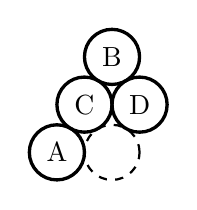
\begin{tikzpicture}[scale=0.7]
          \foreach \x/\y/\n in {0/0/A, 0/2/B, 0/1/C, 1/1/D} {
            \draw[very thick] ({\x + \y/2}, {sqrt(3)/2 * \y}) circle (0.5) node {\n};
          }
          \draw[thick, dashed] (1, 0) circle (0.5);
        \end{tikzpicture}
      }
      child {
        node {
          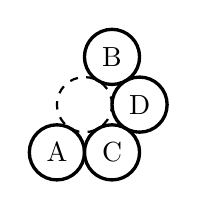
\begin{tikzpicture}[scale=0.7]
            \foreach \x/\y/\n in {0/0/A, 0/2/B, 1/0/C, 1/1/D} {
              \draw[very thick] ({\x + \y/2}, {sqrt(3)/2 * \y}) circle (0.5) node {\n};
            }
            \draw[thick, dashed] (0.5, {sqrt(3)/2}) circle (0.5);
          \end{tikzpicture}
        }
      }
      child {
        node {
          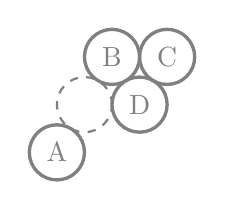
\begin{tikzpicture}[scale=0.7]
            \foreach \x/\y/\n in {0/0/A, 0/2/B, 1/2/C, 1/1/D} {
              \draw[gray, very thick] ({\x + \y/2}, {sqrt(3)/2 * \y}) circle (0.5) node {\n};
            }
            \draw[gray, thick, dashed] (0.5, {sqrt(3)/2}) circle (0.5);
          \end{tikzpicture}
        }
        child {
          node {
            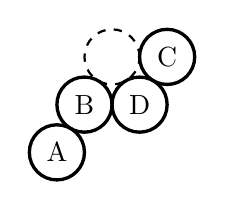
\begin{tikzpicture}[scale=0.7]
              \foreach \x/\y/\n in {0/0/A, 0/1/B, 1/2/C, 1/1/D} {
                \draw[very thick] ({\x + \y/2}, {sqrt(3)/2 * \y}) circle (0.5) node {\n};
              }
              \draw[thick, dashed] (1, {sqrt(3)}) circle (0.5);
            \end{tikzpicture}
          }
        }
        child {
          node {
            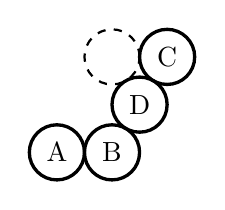
\begin{tikzpicture}[scale=0.7]
              \foreach \x/\y/\n in {0/0/A, 1/0/B, 1/2/C, 1/1/D} {
                \draw[very thick] ({\x + \y/2}, {sqrt(3)/2 * \y}) circle (0.5) node {\n};
              }
              \draw[thick, dashed] (1, {sqrt(3)}) circle (0.5);
            \end{tikzpicture}
          }
        }
        child {
          node {
            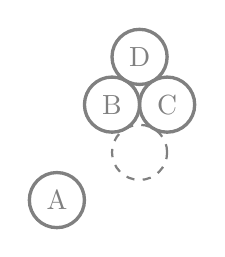
\begin{tikzpicture}[scale=0.7]
              \foreach \x/\y/\n in {0/0/A, 0/2/B, 1/2/C, 0/3/D} {
                \draw[gray, very thick] ({\x + \y/2}, {sqrt(3)/2 * \y}) circle (0.5) node {\n};
              }
              \draw[gray, thick, dashed] (1.5, {sqrt(3)/2}) circle (0.5);
            \end{tikzpicture}
          }
          child {
            node {
              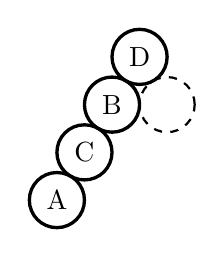
\begin{tikzpicture}[scale=0.7]
                \foreach \x/\y/\n in {0/0/A, 0/2/B, 0/1/C, 0/3/D} {
                  \draw[very thick] ({\x + \y/2}, {sqrt(3)/2 * \y}) circle (0.5) node {\n};
                }
                \draw[thick, dashed] (2, {sqrt(3)}) circle (0.5);
              \end{tikzpicture}
            }
          }
        }
      }
    };
  \end{tikzpicture}

  \caption{
    All connected configurations of $4$ coins. Six out of the seven possible
    polyhexes are present.
  }
\end{figure}
\begin{question}
  In general, given $n$ coins starting in a ``spiral'' configuration, how many
  polyhexes can be reached by the above procedure?
\end{question}

\begin{related}
  \item What if this is done with hyperspheres in $\mathbb{R}^d$?
  \item Is there a sensible way to categorize non-connected configurations?
  \item Which polyhexes require the greatest amount of moves?
\end{related}
\begin{references}
  \item \url{https://en.wikipedia.org/wiki/Polyhex_(mathematics)}
\end{references}
\end{document}
